\chapter{Multimodal face-evoked responses \label{Chap:data:multimodal}}


\section{Overview}

This dataset contains EEG, MEG, functional MRI and structural MRI data on the same subject within the same paradigm, which allows a basic comparison of faces versus scrambled faces.

It can be used to demonstrate, for example, 3D source reconstruction of various electrophysiological measures of face perception, such as the "N170" evoked response (ERP) recorded with EEG, or the analogous "M170" evoked field (ERF) recorded with MEG. These localisations are informed by the anatomy of the brain (from the structural MRI) and possibly by functional activation in the same paradigm (from the functional MRI).

The demonstration below involves localising the N170 using a distributed source method (called an "imaging" solution in SPM). The data can also be used to explore further effects, e.g. induced effects (Friston et al, 2006), effects at different latencies, or the effects of adding fMRI constraints on the localisation.

The EEG data were acquired on a 128 channel ActiveTwo system; the MEG data were acquired on a 275 channel CTF/VSM system; the sMRI data were acquired using a phased-array headcoil on a Siemens Sonata 1.5T; the fMRI data were acquired using a gradient-echo EPI sequence on the Sonata. The dataset also includes data from a Polhemus digitizer, which are used to coregister the EEG and the MEG data with the structural MRI.

Some related analyses of these data are reported in Henson et al (2005a, 2005b, 2007), Kiebel and Friston (2004) and Friston et al (2006).

Most of the analysis below can be done in Matlab7.1 and up. However, recoding condition labels using GUI requires features of SPM8 only available in Matlab7.3 and up. Signal processing toolbox is required for filtering and downsampling steps. 

\section{Paradigm and Data}

The basic paradigm involves randomised presentation of at least 86 faces and 86 scrambled faces (Figure~\ref{fig_32_1}), based on Phase 1 of a previous study by Henson et al (2003). The scrambled faces were created by 2D Fourier transformation, random phase permutation, inverse transformation and outline-masking of each face. Thus faces and scrambled faces are closely matched for low-level visual properties such as spatial frequency power density. Half the faces were famous, but this factor is collapsed in the current analyses. Each face required a four-way, left-right symmetry judgment (mean RTs over a second; judgments roughly orthogonal to conditions; reasons for this task are explained in Henson et al, 2003). The subject was instructed not to blink while the fixation cross was present on the screen.


\begin{figure}
\begin{center}
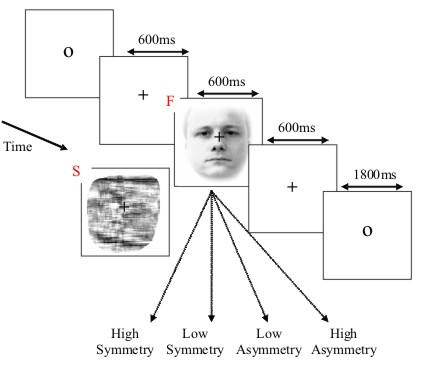
\includegraphics[width=100mm]{multimodal/figures/figure_32_1}
\caption{\em One trial in the experimental paradigm: Trials involved either a Face (F) or Scrambled face (S). \label{fig_32_1}}
\end{center}
\end{figure}

\subsection{Structural MRI}

The T1-weighted structural MRI of a young male was acquired on a 1.5T Siemens Sonata via an MDEFT sequence with resolution $1 x 1 x 1 mm^3$ voxels, using a whole-body coil for RF transmission and an 8-element phased array head coil for signal reception.

The images are in Analyze format in the sMRI sub-directory, consisting of two files:
\begin{verbatim}
    sMRI/sMRI.img
    sMRI/sMRI.hdr
\end{verbatim}
The structural was manually-positioned to match roughly Talairach space, with the origin close to the Anterior Commissure, which produced the associated SPM Matlab file:
\begin{verbatim}
    sMRI/sMRI.mat
\end{verbatim}
The approximate position of 3 fiducials within this MRI space - the nasion, and the left and right peri-aricular points - are stored in the file:
\begin{verbatim}
    sMRI/smri_fid.txt
\end{verbatim}
These were identified manually (based on anatomy) and are used to define the MRI space relative to the EEG and MEG spaces, which need to be coregistered (see below). It doesn't matter that the positions are approximate, because more precise coregistration is done via digitised surfaces of the scalp ("head shape functions") that were created using the Polhemus 3D digitizer.

\subsection{EEG data}

The EEG data were acquired on a 128-channel ActiveTwo system, sampled at 2048 Hz, plus electrodes on left earlobe, right earlobe, and two bipolar channels to measure HEOG and VEOG. The 128 scalp channels are named: 32 A (Back), 32 B (Right), 32 C (Front) and 32 D (Left). The data acquired in two runs of the protocol is contained in two Biosemi raw data files:
\begin{verbatim}
    EEG/faces_run1.bdf
    EEG/faces_run2.bdf
\end{verbatim}

The EEG directory also contains the following files:
\begin{verbatim}
    EEG/condition_labels.txt
\end{verbatim}
This text file contains a list of condition labels in the same order as the trials appear in the two files (when concatenated) - 'faces' for presentation of faces and 'scrambled' for presentation of scrambled faces. 
The EEG directory also contains the following files:
\begin{verbatim}
    EEG/electrode_locations_and_headshape.sfp
\end{verbatim}
This ASCII file contains electrode locations, fiducials and headshape points measured with Polhemus digitizer.
The EEG directory also contains the following files:


The 3 fiducial markers were placed approximately on the nasion and peri-aricular points and digitised by the Polhemus digitizer. The digitizer was also used to locate the position of each electrode (in the \verb!electrode_locations.sfp! file), and to record multiple points on the surface of the  subject's scalp and nose (the "head shape function" in the \verb!headshape.mat! file). Later, we will coregister the fiducial points and the head shape to map the electrode positions in the "Polhemus space" to the "MRI space".

\subsection{MEG data \label{meg}}

The MEG data were acquired on a 275 channel CTF/VSM system, using second-order axial gradiometers and synthetic third gradient for denoising and sampled at 480 Hz. Two runs of the protocol have been saved in two CTF datasets (each one is a directory with multiple files) 
\begin{verbatim}
    MEG/SPM_CTF_MEG_example_faces1_3D.ds
    MEG/SPM_CTF_MEG_example_faces2_3D.ds
\end{verbatim}
The MEG data also contains a \verb!headshape.mat! file, containing the headshape recorded during the MEG experiment withPolhemus digitizer.

The locations of the 3 fiducials in the \verb!headshape.pol! file are the same as the positions of 3 "locator coils" the locations of which are measured by the CTF machine, and used to define the coordinates (in "CTF space") for the location of the 275 sensors.

\subsection{fMRI data}

The fMRI data were acquired using a Trajectory-Based Reconstruction (TBR) gradient-echo EPI sequence (Josephs et al, 2000) on a 1.5T Sonata. There were 32, 3mm slices of 3x3 mm2 pixels, acquired in a sequential descending order with a TR of 2.88s. There are 215 images in the 'Scans' sub-directory (5 initial dummy scans have been removed), each consisting of an Analyze image and header file:
\begin{verbatim}
    fMRI/Scans/fM*.img  
    fMRI/Scans/fM*.hdr
\end{verbatim}
Also provided are the onsets of faces and scrambled faces (in units of scans) in the Matlab file:
\begin{verbatim}
    fMRI/onsets.mat 
\end{verbatim}
and the SPM "Job" files (see Section~\ref{fMRI}):
\begin{verbatim}
    fMRI/realign_job.mat
    fMRI/slicetime_job.mat
    fMRI/smooth_job.mat
    fMRI/stats_job.mat
\end{verbatim}

\section{Getting Started}

You need to start SPM8 and toggle "EEG" as the modality (bottom-right of SPM main window), or start SPM8 with \verb!spm eeg!. In order for this to work you need to ensure that the main SPM directory is on your Matlab path.


\section{EEG analysis}

\subsection{Convert}

Press the \textsc{Convert} button and select the \texttt{faces_run1.bdf} file. At the prompt ``Define settings?'' select ``just read''.
SPM will now read the original Biosemi format file and create an SPM combatible data file, called \texttt{spm8\_faces_run1.bdf} and \texttt{spm8\_faces_run1.bdf} in the current Matlab directory. You can either change directory to where the EEG files are or perhaps more conveniently create a new directory for your analysis results and make it Matlab's current directory before staring. If you want to repeat the analysis later you can always erase this directory without affecting the original data files. After the conversion is complete the data file will be automatically opened in SPM8 reviewing tool. By default you will see the 'info' pad. At the top of the window there is some basic information about the file. Below it you will see several clickable tabs with additional information. The 'history' tab lists the processing steps that have been applied to the file. At this stage there is only one such step - conversion. The 'channels' tab lists the channels in the file and their properties, the trial tab lists the trials or in the case of a continuous file all the triggers (events) that have been recorded. The 'inv' tab is used for reviewing the inverse solutions and is not relevant for the time being. Nothe that the detailed information in the tabs will not be available for Matlab 7.1.  At the top of the window there is another set of tabs. If you click on the 'EEG' tab you will see the raw EEG traces. The all look unusually flat because the continuous data we have just converted contains very low frequencies and constand baseline shifts. Therefore, if we try to view all the channels together, this can only be done with very low gain. 
If you press the 'intensity rescaling' button (with arrows pointing up and down) several times you will start seeing EEG activity in a few channels but the other channels will not be visible as they will go out of range. You can also use the controls at the bottom of the window to scroll through the recording. As you do this, you will see vertical lines indicating triggers, in our case presentation of visual stimuli. 

\subsection{Downsample}
Here, we will downsample the data in time. This is useful when the data were acquired like ours with a high sampling rate of 2048 Hz. This is an unnecessarily high sampling rate for a simple evoked response analysis, and we will now decrease the sampling rate to 200 Hz, thereby reducing the file size by more than ten fold and greatly speeding up the subsequent processing steps. This step requires the signal processing toolbox. Select \textsc{Downsample} from the ``Other'' drop-down menu and select the \texttt{spm8\_faces_run1.mat} file. Choose a new sampling rate of 200 (Hz). The progress bar will appear and the resulting data will be saved to files \texttt{dspm8\_faces_run1.mat} and \texttt{dspm8\_faces_run1.dat}. Note that this datasets and other intermediate datasets created during preprocessing will not be automatically opened in the reviewing tool, but you can always review them by selecting \verb!M\EEG! from the 'Display' drop down menu and choosing the corresponding .mat file.


\subsection{Montage}

In this step, we will identify the VEOG and HEOG channels, remove several channels that don't carry EEG data and are of no importance to the following and convert the 128 EEG channels to 'average reference' by subtracting the mean of all the channels from each channel. We generally recommend to remove all data channels that are no longer needed because it will reduce the total file size and conversion to average reference is necessary at present to for source modelling to work correctly.  To do so, we use the \textsc{mont ge} tool in SPM, which is a general approach for pre-multiplying the data matrix (channels $\times$ time) by another matrix that linearly weights all channel data. This provides a very general method for data transformation in M/EEG analysis.

The appropriate montage-matrix can be derived as follows.
In our case, we would like to only keep channels 1 to 128. In addition, there were four EOG channels (131, 132, 135, 136), where the VEOG is computed as the difference between channels 131 and 132, and the VEOG by the difference between channels 135 and 136. This matrix can be specified in SPM by either using a graphical interface, or by supplying the matrix saved in a file. We will do the latter. The script to generate this file can be found in the \texttt{example\_scripts} folder: \texttt{faces\_eeg\_montage.m}. Copy this script into the directory with  \texttt{dspm8\_faces_run1.mat} file and run it. This will generate a file named \texttt{faces\_eeg\_montage.mat}.

You now call the montage function by choosing \textsc{Montage} in the ``Other'' drop-down menu and:
\begin{itemize}
\item{Select the M/EEG-file \texttt{dspm8\_faces_run1.mat}}
\item{`How to specify the montage ?' Answer ``file''.}
\item{Then select the generated \texttt{faces\_eeg\_montage.mat} file}
\item{``Keep the other channels?'' : ``No''}
\end{itemize}
This will remove the uninteresting channels from the data. The progress bar appears and SPM will generate two new files \texttt{Mdspm8\_faces_run1.mat} and \texttt{Mdspm8\_faces_run1.dat}.

\subsection{Epoch}
To epoch the data click on \textsc{Epoching}. Select the \texttt{Mdspm8\_faces_run1.mat} file. Choose the peri-stimulus time window, first the start \texttt{-200}, then the end \texttt{600} ms. Choose 1 conditions. There is no information in the file at this stage to distinguish between faces and scrambled faces. We will add this information at a later stage. You can give this condition any label, for instance ``stim''. A GUI pops up which gives you a complete list of all events in the EEG file. Each event has type and value which might mean different things for different EEG and MEG systems. So you should be familiar with your particular system to find the right trigger for epoching. In our case it is not very difficult as all the events but one appear only once in the recording, whereas the event with type 'STATUS' and value 1 appears 172 times which is exactly the number of times a visual stimulus was presented. Select this event and press OK. Answer two times ``no'' to the questions ``review individual trials'', and ``save trial definitions''. The progress bar will appear and the epoched data will be saved to files \texttt{eMdspm8\_faces_run1.mat} and \texttt{eMdspm8\_faces_run1.dat}. The epoching function also performs baseline correction by default (with baseline -200 to 0ms). Therefore, in the epoched data the large channel-specific DC-shifts are removed and it is finally possible to see the EEG data clearly in the reviewing tool.


\subsection{Reassignment of trial labels}
Open the file \texttt{eMdspm8\_faces_run1.mat} in the reviewing tool. The first thing you will see is that in the history tab there are now 4 processing steps. Now switch to the 'trials' tab. You will see a table with 172 rows - exatly the number of events we selected before. In the first column the label 'stim' appears in every row. What we would like to do now is change this label to 'faces' or 'scrambled' where appropriate. We should first open the file \verb!condition_labels.txt! with any text editor, such as Matlab editor or Windows notepad. In this file there are exactly 172 rows with either 'faces' or 'scrambled' in each row. Select and copy all the rows (Ctrl-A, Ctrl-C on Windows). Then go back to SPM and the trials tab. Place the cursor in the first row and first column cell with the 'stim' label and paste the copied labels (Ctrl-V). The new labels should now appear for all rows. Press the 'update' button above the table and then the 'SAVE' button at the top right corner of the window. The new labels are now saved in the dataset.  


\subsection{Using the history and object methods to preprocess the second file}
At this stage we need to repeat the preprocessing steps for the second file \texttt{faces_run2.bdf}. You can do it by going back to the 'Convert' section and repeating all the steps for this file, but there is a more efficient way. If you have been following the instructions until now the file \texttt{eMdspm8\_faces_run1.mat} should be open in the reviewing tool. If it is not the case, open it. Go to the 'history' tab and press the 'Save as script' button. This button should be available even for the versions of Matlab where the detailed history information cannot be displayed. A dialog will appear asking for the name of the Matlab script to save. Lets call it \texttt{preprocess.m}. Then there will be another dialogue suggesting to select the steps to save in the script. Just press OK to save all the steps. Now open the script in the Matlab editor. You will now need to make some changes to make it work for the second file. Here we suggest the simplest way to do it that does not require familiaty with Matlab programming. But if you are more familar with Matlab you'll definitely be able to do much better job. First, replace all the occurences of 'run1' in the file with 'run2'. You can use the 'Find & Replace' functionalty (Ctrl-F) to do it. Secondly, erase the line starting with \verb!S.timewindow! (line 5). This line defines the time window to read, in this case from the first to the last sample of the first file. The second file is slghtly longer than the first so we should let SPM determine the right time window automatically. Save the changes and run the script by pressing the 'Run' button or writing 'preprocess' in the command line. SPM will now automatically perform all the steps we have done before using the GUI. This is a very easy way for you to start processing your data automatically once you come up with the right sequence of steps for one file. After the script finishes running there will be a new set of files in the current directory including \texttt{eMdspm8\_faces_run2.mat} and \texttt{eMdspm8\_faces_run2.dat}. If you open these files in the reviewing tool and go to the 'trials' tab you will see that the trial labels are still 'stim'. The reason for this is that updates done using the reviewing tool are not presently recorded in the history (with the exception of the 'Prepare' interface, see below). You can still do this update automatically and add it to your script. If you write 'D' in the command line just after running the script and press 'Enter' you will see some information about the dataset \texttt{eMdspm8\_faces_run2}. D is an object, this is a special kind of data structure that makes it possible to keep different kinds of related information (in our case all the properties of our dataset) and define generic ways of manipulating these properties. For instance we can use the command:
\begin{verbatim}
D = conditions(D, [], importdata('condition_labels.txt'));save(D);
\end{verbatim}
to update the trial labels using information imported from the \texttt{condition_labels.txt}. You might need to write the full path to this text file inside the single quotes or copy the file to the directory where you are working for this command to work. 'conditions' is a 'method', special function that knows where to store the labels in the object. All the methods take the M\EEG object (usually called D in SPM by convention) as the first argument. The second argument is a list of indices of trials for which we want to change the label. We specify an empty matrix which is interpreted as 'all'. The third argument is the new labels which are imported from the text file using Matlab built-in function. We then save the updates dataset on disk using the 'save' method. If you now write \verb!D.conditions! or \verb!conditions(D)! (which are two equivalent ways of calling the 'conditions' method with just D as an argument), you should see a list of 172 labels, either 'faces' or 'scrambled'. If you add the commands above at the end of your automatically generated script, you can run it again and this time the output will have the right labels. 

\subsection{Merge}
We will now merge the two epoched files we have generated until now and continue working on the merged file. Select the 'Merge' command from the 'Other' drop-down menu. In the selection window that comes up click on \texttt{eMdspm8\_faces_run1.mat} and \texttt{eMdspm8\_faces_run2.mat}. Press 'done'. Answer 'Leave as they are' to 'What to do with condition labels?'. This means that the trial labels we have just specified will be copied as they are to the merged file. A new dataset will be generated called \texttt{ceMdspm8\_faces_run1}.

\subsection{Prepare}
In this section we will add the separately measured electrode locations and headshape points to our merged dataset. In principle, this step is not essential for further analysis because SPM8 automatically assigns electrode locations for commonly used EEG caps and the Biosemi 128 cap is one of these. Thus, default electrode locations are present in the dataset already after conversion. But since these locations are based on channel labels they may not be precise enough and in some cases may be completely wrong because sometimes electrodes are not placed in the correct locations for the corresponding channel labels. This can be corrected by importing individually measured electrode locations. Select 'Prepare' from the 'Other' menu and in the file selection window select \texttt{ceMdspm8\_faces_run1.mat}. A menu will appear at the top of SPM's interactive window (small window at the bottom left). In the 'Sensors' submenu choose 'Load EEG sensors'/'Convert locations file'. In the file selection window choose the \texttt{electrode_locations_and_headshape.sfp} file. From '2D projection' submenu select 'Project 3D (EEG)'. 2D channel layout will appear in the graphics window. Select 'Apply' from '2D Projection' and 'Save' from 'File' submenu. Note that the same functionality can also be accessed from the reviewing tool by pressing the 'Prepare SPM file' button.

\subsection{Artefact rejection}
Here we will use SPM8 artefact detection functionality to exclude from analysis trials contaminated with large artefacts. Press the 'Artefacts' button. A window of SPM8 batch interface will open. You might be already familiar with this interface from other SPM8 functions. It is also possible to use the batch interface to run the preprocessing steps that we have performed until now, but for artefact detection this is the only graphical interface. Click on 'File name' and select the \verb!ceMdspm8_faces_run1.mat! file.  Double click 'How to look for artefacts' and a new branch will appear. It is possible to define several sets of channels to scan and several different methods for artefact detection. We will use simple thresholding applied to all channels. Click on 'Detection algorithm' and select 'Threshold channels' in the small window below. Double click on 'Threshold' and enter 200 (in this case uV). The batch is now fully configured. Run it by pressing the green button at the top of the batch window. 

This will detect trials in which the signal recorded at any of the channels exceeds 200 microvolts (relative to pre-stimulus baseline). These trials will be marked as artefacts. Most of these artefacts occur on the VEOG channel, and reflect blinks during the critical time window. The procedure will also detect channels in which there are a large number of artefacts (which may reflect problems specific to those electrodes, allowing them to be removed from subsequent analyses).

In this case, the Matlab window will show:
\begin{verbatim}
    There isn't a bad channel.
     39 rejected trials: 38   76   82   83   86   88   89   90   92   93   94   96   98   99  100  101  104  105  106  107  108  112  117  118  119  122  124  126  130  137  139  159  173  221  266  268  279  281  298
\end{verbatim}
(leaving 305 valid trials). A new file will also be created, \verb!aceMdspm8_faces_run1.mat!.

\subsection{Exploring the M/EEG object}
We can now review the preprocessed dataset from the Matlab command lineby typing:
\begin{verbatim}
    D = spm_eeg_load
\end{verbatim}
and selecting the \verb!aceMdspm8_faces_run1.mat! file. This will print out some basic information about the M/EEG object D that has been loaded into Matlab workspace.
\begin{verbatim}
SPM M/EEG data object
Type: single
Transform: time
2 conditions
130 channels
161 samples/trial
344 trials
Sampling frequency: 200 Hz
Loaded from file  D:\Data\Multimodal\EEG\spm\aceMdspm8_faces_run1.mat

Use the syntax D(channels, samples, trials) to access the data
Type "methods('meeg')" for the list of methods performing other operations with the object
Type "help meeg/method_name" to get help about methods
\end{verbatim}

Note that the data values themselves are memory-mapped from the \verb!aceMdspm8_faces_run1.dat! and can be accessed by indexing the D object (e.g, D(1,2,3) returns the field strength in the first sensor at the second sample point during the third trial). You will see that there are 344 trials (D.ntrials). Typing D.conditions will show the list of condition labels consisting of 172 faces ('faces') and 172 scrambled faces ('scrambled'). D.reject will return a 1x344 vector of ones (for rejected trials) and zeros (for retained trials). D.condlist will display a list of unique condition labels. The order of this list is important for some because every time SPM needs to process the conditions in some order, this will be the order. If you type D.chanlabels, you will see the order and the names of the channels. D.chantype will display the type for each channel (in this case either 'EEG' or 'EOG'). D.size will show the size of the data matrix, [130 161 344] (for channels, samples and trials respectively). The size of each dimension separately can be accessed by D.nchannels, D.nsamples and D.ntrials. Note that although the syntax of these commands is similar to the commands used for accessing the fields of struct data type in Matlab what's actually happening is that these commands envoke special functions called 'methods' and these methods actually collect and return the requested information from the internal data structure of the D object. The internal structure is not accessible directly when working with the object. This mechanism greatly enhances the robustness of SPM code. For instance you don't need to check whether some field is present in the internal structure. The methods will allways do it automatically or return some default result in the information is missing without causing an error.


\subsection{Basic ERPs}

* Press the 'Averaging' button and select the \verb!aceMdspm8_faces_run1.mat! file. At this point you can perform either orinary averaging or 'robust averaging' (Wager et al.). Robust averaging makes it possible to supress artefacts automatically without rejecting trials or channels compltely, but just the contaminated parts. Thus, in principle we could do robust averaging without rejecting trials with eye blinks and this is something you can do as an exercise and see how much difference the artefact rejection makes with ordinary averaging vs. robust averaging. For robust averaging answer 'yes' to 'Use robust averaging?'. Answer 'yes' to 'Save weights', and 'Compute weights by condition' and press 'Enter' to accept the default 'Offset of the weighting function'. A new dataset will be generated \verb!maceMdspm8_faces_run1! ("m" for "mean") and automatically opened in the reviewing tool so that you can examine the ERP. There will also be an additional dataset named \verb!WaceMdspm8_faces_run1! this dataset will contain instead of EEG data the weights used by robust averaging. This is useful to see what was suppressed and whether there might be some condition-specific bias that could affect the results. 

* Press the 'Filtering' button, select the \verb!maceMdspm8_faces_run1.mat! file, select 'lowpass', and enter 40 (Hz) as the cutoff. This smooths the data to 40Hz, producing the file \verb!fmaceMdspm8_faces_run1.mat! (using zero-phase-shift forward and reverse  digital filtering with a 5th-order Butterworth filter)\footnote{Note that (lowpass) filtering short epochs like this is not necessarily a good idea, since ringing or "end-effects" can result at the start and end of the epoch. Filtering is normally better performed on continuous data (or longer epochs). The filtering performed here is simply to demonstrate the option and for display purposes (though the averaging process also tends to act like a lowpass filter anyway).}.

* Select "Contrast" from the "Other..." pulldown menu on the SPM window (or type \verb!spm_eeg_weight_epochs! in the Matlab window). This function creates linear contrasts of ERPs/ERFs. Select the \verb!fmaceMdspm8_faces_run1.mat! file,  enter $[1 -1]$ as the first contrast and label it 'Difference', answer 'yes' to 'Add another',  enter $[1/2 1/2]$ as the second contrast and label it 'Mean'. Press "no" to the question 'Add another' and not to "weight by num replications". This will create new file \verb!wfmaceMdspm8_faces_run1.mat!, in which the first trial-type is now the differential ERP between faces and scrambled faces, and the second trial-type is the average ERP for faces and scambled faces.

To look at the differential ERP, again press 'Display: M/EEG', and select the \verb!wfmaceMdspm8_faces_run1.mat! file. Switch to the 'EEG' tab and to 'scalp' display by toggling a radio button at the top of the tab. After a short delay, the Graphics window should show the ERP for each channel (for Trial 1 - the'Difference' condition). Hold SHIFT and select Trial 2 to see both conditions superimposed. Then click on the zoom button and then on one of the channels (e.g, 'B9' on the bottom right of the display) to get a new window with the data for that channel expanded, as in Figure~\ref{fig_32_4}.

\begin{figure}
\begin{center}
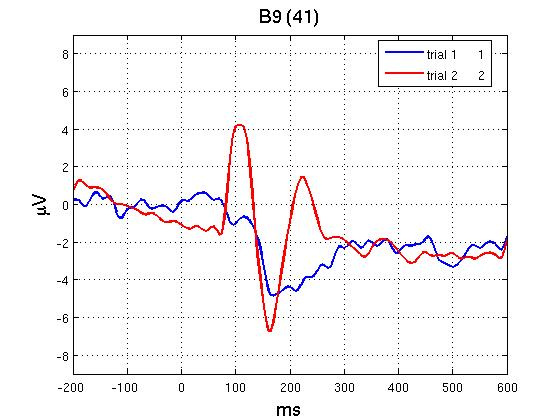
\includegraphics[width=100mm]{multimodal/figures/figure_32_4}
\caption{\em  Average (red) and differential (blue) ERPs for faces and scrambled faces at channel B9 in wfmaceMdspm8_faces_run1.mat. \label{fig_32_4}}
\end{center}
\end{figure}

The green line shows the average ERP evoked by faces and scrambled faces (at this occipitotemporal channel). A P1 and N1 are clearly seen. The blue line shows the differential ERP between faces and scrambled faces. This is approx zero around the P1 latency, but negative around the N1 latency. The latter likely corresponds to the "N170" (Henson et al, 2003). We will try to localise the cortical sources of the P1 and N170 in Section~\ref{3D}.

To see the topography of the differential ERP, click on Trial 1 again, press the "topography" button at the top of the window and scroll to 180ms for the latency to produce Figure~\ref{fig_32_5}.

\begin{figure}
\begin{center}
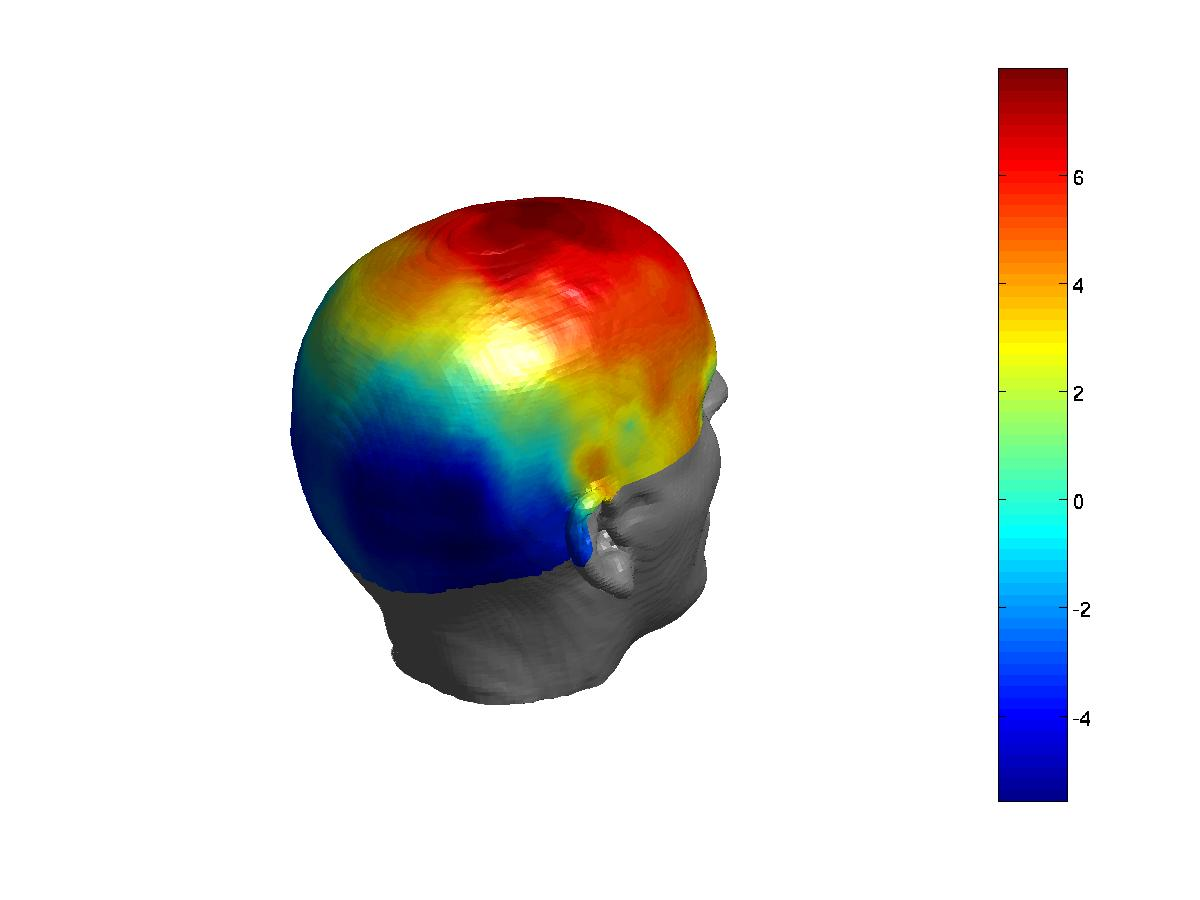
\includegraphics[width=100mm]{multimodal/figures/figure_32_5}
\caption{\em 3D topography for faces minus scrambled faces at 180ms. \label{fig_32_5}}
\end{center}
\end{figure}


\subsection{3D SPMs (Sensor Maps over Time) \label{3DSPM}}

One novel feature of SPM is the ability to use Random Field Theory to correct for multiple statistical comparisons across N-dimensional spaces. For example, a 2D space representing the scalp data can be constructed by flattening the sensor locations (using the 2D layout we created earlier) and interpolating between them to create an image of MxM pixels (when M is user-specified, eg M=32). This would allow one to identify locations where, for example, the ERP amplitude in two conditions at a given timepoint differed reliably across subjects, having corrected for the multiple t-tests performed across pixels. That correction uses Random Field Theory, which takes into account the spatial correlation across pixels (i.e, that the tests are not independent). This kind of analysis is described earlier in the SPM manual, where a 1st-level design is used to create the images for a given weighting across timepoints of an ERP/ERF, and a 2nd-level design can then be used to test these images across subjects.

Here, we will consider a 3D example, where the third dimension is time, and test across trials within the single subject. We first create a 3D image for each trial of the two types, with dimensions MxMxS, where S=161 is the number of samples. We then take these images into an unpaired t-test across trials (in a 2nd-level model) to compare faces versus scrambled faces. We can then use classical SPM to identify locations in space and time in which a reliable difference occurs, correcting across the multiple comparisons entailed. This would be appropriate if, for example, we had no a priori knowledge where or when the difference between faces and scrambled faces would emerge\footnote{Note that the 2D location in sensor space for EEG will depend on the choice of montage.}.

* Select the "Convert to images" option in the "Other..." menu in the Matlab window, and select the \verb!aceMdspm8_faces_run1.mat! file. You will then be prompted for "output image dimensions", for which you can accept the default of 32 (leading to a 32x32 pixel space). It will then ask whether you want to interpolate or mask out bad channels, for which you an select interpolate (though it will make no difference here because there are no bad channels).

This will take some time as it writes out an image for each trial (except rejected trials), in a new directory called \verb!aceMdspm8_faces_run1!, which will itself contain two subdirectories, one for each trialtype. In each trialtype subdirectory there will be image and header files for each non-rejected trial of that type, e.g, trial0002.img/hdr. You can press "Display: images" to view one of these images - it will have dimensions 32x32x161(x1), with the origin set at [16 18.6 40] (where 40 samples is 0ms), as in Figure~\ref{fig_32_6}.


\begin{figure}
\begin{center}
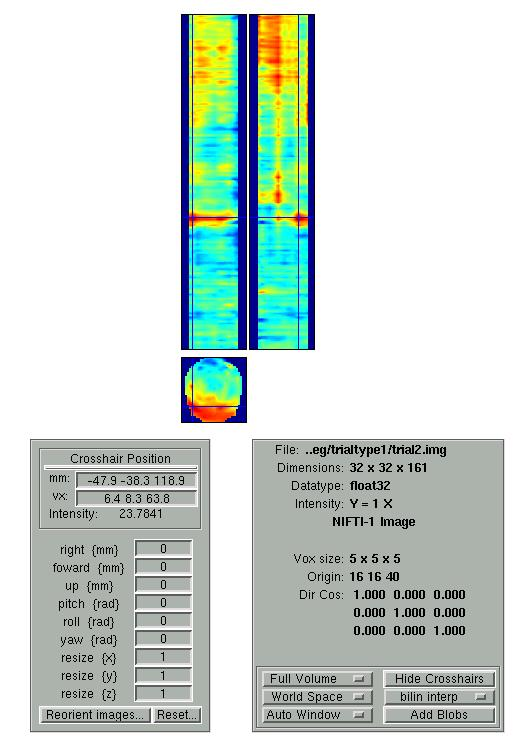
\includegraphics[width=100mm]{multimodal/figures/figure_32_6}
\caption{\em  3D image for trial 2 of aceMdspm8_faces_run1.mat. The bottom image is a square 2D x-y space interpolated from the flattened electrode locations (at one point in time). The two top images are sections through x and y respectively, now expressed over time (vertical (z) dimension). (Colormap changed to 'jet').\label{fig_32_6}}
\end{center}
\end{figure}

To perform statistics on these images, first create a new directory, eg. mkdir XYTstats.

* Then press the "specify 2nd level" button,  select "two-sample t-test" (unpaired t-test), and define the images for "group 1" as all those in the subdirectory "type_faces" (using right mouse, and "select all") and the images for "group 2" as all those in the subdirectory "type_scrambled". Finally, specify the new XYTstats directory as the output directory, and press "run"\footnote{Note that we can use the default "nonsphericity" selections, i.e, that the two trial-types may have different variances, but are uncorrelated.}.



This will produce the design matrix for a two-sample t-test.

* Then press "Estimate", and when it has finished, press "Results" and define a new F-contrast as [1 -1] (for help with these basic SPM functions, see eg. chapter 26). Keep the default contrast options, but threshold at $p<.05$ FWE corrected for the whole "image". Then press "volume", and the Graphics window should now look like that in Figure~\ref{fig_32_7} (ignore the outline of the brain in the MIP!).

This will reveal "regions" within the 2D sensor space and within the -200ms to 600ms epoch in which faces and scrambled faces differ reliably, having corrected for multiple F-tests across pixels/time. There are a number of such regions, but we will concentrate on the first two (largest ones), with cluster maxima of  [25 -55 200] and [10 5 160]. An F-test was used because the sign of the difference reflects the polarity of the ERP difference, which is not of primary interest (and depends on the choice of reference; see footnote 6). Indeed, if you plot the contrast of interest from the cluster maxima, you will see that the difference is negative for the first cluster (which is located posteriorly) but positive for the second cluster (which is more central, close to Cz). This is consistent with the polarity of the differences in Figure~\ref{fig_32_3}\footnote{With the current reference, the former likely corresponds to the "N170", while the latter likely corresponds to the "VPP" (though we have no evidence here for a dissociation between them).}.

If one had more constrained a priori knowledge about where and when the N170 would appear, one could perform an SVC based on, for example, a box around posterior channels and between 150 and 200ms poststimulus.

\begin{figure}
\begin{center}
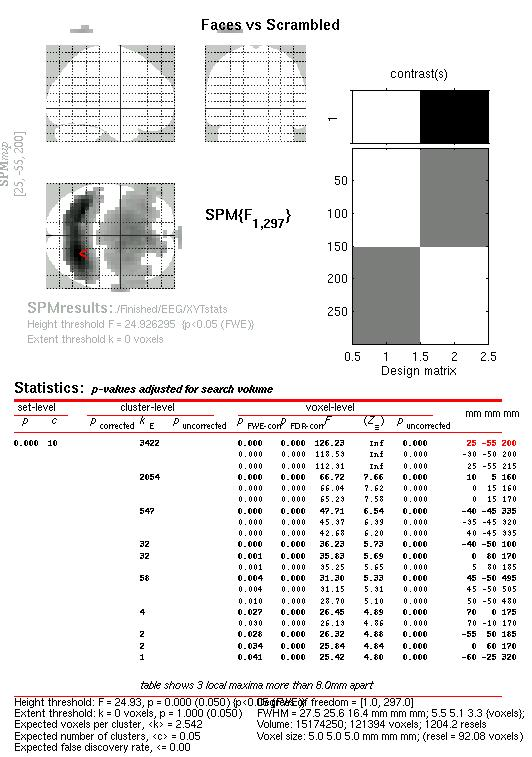
\includegraphics[width=100mm]{multimodal/figures/figure_32_7}
\caption{\em 3D sensor-time SPM{F} at $p<.05$ FWE corrected for the amplitude difference between face and scrambled face trials. Note that the brain outline in the MIP should be ignored. The x, y coordinates refer to arbitrary units in the 32x32 electrode plane (origin = [16 16]); the z coordinate refers to peristimulus time in ms (to the nearest sampling of 5ms). \label{fig_32_7}}
\end{center}
\end{figure}

\subsection{3D "imaging" reconstruction \label{3D}}

Here we will demonstrate a distributed source reconstruction of the N170 differential evoked response between faces and scrambled faces, using a grey-matter mesh extracted from the subject's MRI, and the Multiple Sparse Priors (MSP) method in which multiple constraints on the solution can be imposed (Phillips et al, 2002; Mattout et al, 2005; Henson et al, 2007; Friston et al, in press-a).
* Press the '3D source reconstruction' button, and press the "load" button at the top of the new window. Select the \verb!wfmaceMdspm8_faces_run1.mat! file and type a label (eg "N170") for this analysis\footnote{Note that no new M/EEG files are created during each stage of the 3D reconstruction; rather, each step involves updating of the cell-array field D.inv, which will have one entry per analysis performed on that dataset (e.g, D.inv\{1\} in this case).}.

* Press the 'MRI' button, select the smri.img file within the sMRI sub-directory, press the "Imaging" button, and select 'normal' for the cortical mesh.

The "imaging" option corresponds to a distributed source localisation, where current sources are estimated at a large number of fixed points (8196 here) within a cortical mesh, rather than approximated by a small number of equivalent dipoles (the ECD option). The imaging or distributed approach is better suited for group analyses and probably for later components; the ECD approach may be better suited for very early sensory components (when only small parts of the brain are active), or for DCM models of a small number of regions (Kiebel et al, 2006).

The first time you use a particular structural image for 3D source reconstruction, it will take some time while the MRI is segmented (and normalisation parameters determined). This will create in the sMRI directory the files \verb!y_smri.nii! and \verb!smri_seg8.mat! for normalisation parameters and 4 GIFTI (.gii) files defining the cortical mesh, inner skull, outer skull and scalp surface. 

When meshing has finished, the cortex (blue), inner skull (red) and scalp (orange) meshes will also be shown in the Graphics window with slices from the sMRI image. This makes it possible to verify that the meshes indeed fit the original image well. The field D.inv\{1\}.mesh field will be updated in matlab. Press "save" in top right of window to update the corresponding mat file on disk.

Both the cortical mesh and the skull and scalp meshes are not created directly from the segmented MRI, but rather are determined from template meshes in MNI space via inverse spatial normalisation (Mattout et al, in press).

* Press the 'Co-register' button. You will be asked for each of the 3 fiducial points to specify its location on the MRI images. This can be done by  selecting a corresponding point from a hard-coded list ('select'). These points are inverse transformed for each individual image using the same deformation field that is used to create the meshes. The other two options are typing the MNI coordinates for each point ('type') or clicking on the corresponding point in the image ('click'). We will use the 'select' option and just press OK for each point as SPM automatically selects a point with the same name. Answer 'yes' to 'Use headshape points?'.

This stage coregisters the EEG sensor positions with the structural MRI and cortical mesh, via an approximate matching of the fiducials in the two spaces, followed by a more accurate surface-matching routine that fits the head-shape function (measured by Polhemus) to the scalp that was created in the previous meshing stage via segmentation of the MRI. When coregistration has finished, the field D.inv\{1\}.datareg will be updated in matlab. Press "save" in top right of window to update the corresponding mat file on disk. Finally, a figure like that in Figure~\ref{fig_32_8} will also be produced, which you can rotate with the mouse (using the Rotate3D Matlab Menu option) to check all sensors.


\begin{figure}
\begin{center}
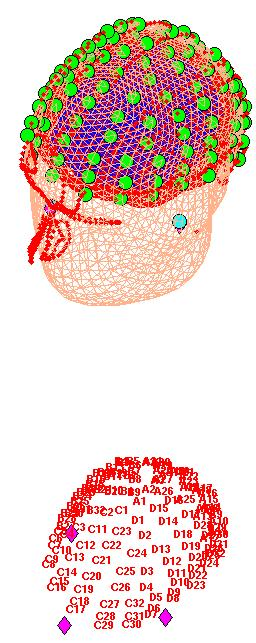
\includegraphics[width=70mm]{multimodal/figures/figure_32_8}
\caption{\em  Graphical output of Co-registration of EEG data, showing (upper panel) cortex (blue), inner skull (red) and scalp (black) meshes, electrode locations (green), MRI/Polhemus fiducials (cyan/magneta), and headshape (red dots).\label{fig_32_8}}
\end{center}
\end{figure}

\noindent * Press 'Forward Model', and select "EEG BEM". The first time you do this, there will be a lengthy computation and a large file \verb!smri_EEG_BEM.mat! will be saved in the sMRI directory containing the parameters of the boundary element model (BEM). In the graphics window the BEM meshes will be displayed with the EEG sensors marked as asterisks. This display is the final quality control before the model is used for lead field computation.

* Press 'Invert', select "Imaging" (i.e, a distributed solution rather than DCM; Kiebel et al, 2006), select "yes" to include all conditions (i.e, both the differential and common effects of faces and scrambled faces) and then "Standard" to use the default settings.

By default the MSP method will be used. MSP stands for "Multiple Sparse Priors", and has been shown to be superior to standard minimum norm (the alternative MNM option) or a maximal smoothness solution (like LORETA; the COH option) - see Friston et al (in press-a). Note that by default, MSP uses a "Greedy Search" (GS) (Friston et al, in press-b), though the standard ReML (as used in Friston et al, in press-a) can also be selected (ARD).

The "Standard" option uses default values for the MSP approach (to customise some of these parameters, press "Custom" instead). 

At the first stage of the inversion lead fields will be computed for all the mesh verticed and saved in the file \verb!SPMgainmatrix_wfmaceMdspm8_faces_run1_1.mat!. Then the actual MSP algorithm will run and the summary of the solution will be displayed in the graphics window.

* Press "save" to save the results. You can now explore the results via the 3D reconstruction window. If you type 165 into the box in the bottom right (corresponding to the time in ms) and press "mip", you should see an output like in~\ref{fig_32_9}. This fit explains approx 97\% of the data.

Note the hot-spots in the fusiform. The timecourses come from the peak voxel. The red line shows the condition currently being shown (corresponding to the "Condition 1" toggle bar in the reconstruction window); the grey line(s) will show all other conditions. Condition 1 is the differential evoked responses for faces vs scrambled; if you press the "condition 1" toggle, it will change to Condition 2 (average evoked response for faces and scrambled faces), then press "mip" again and the display will update (note the colours of the lines have now reversed from before, with red now corresponding to average ERP).

If you toggle back to condition 1 and press "movie", you will see the changes in the source strengths for the differential response over peristimulus time (from the limits 0 to 300ms currently chosen by default).

If you press "render" you can get a very neat graphical interface to explore the data (the buttons are fairly self-explanatory). However, we will concentrate on how one might perform statistics (eg with more subjects in a group analysis).


\begin{figure}
\begin{center}
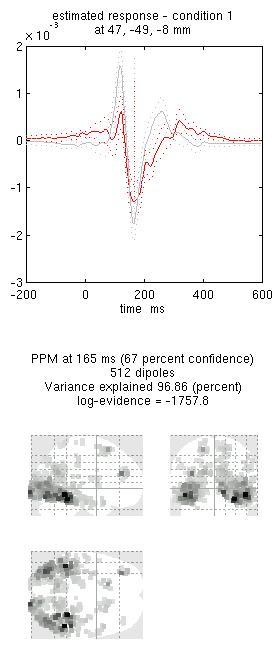
\includegraphics[width=90mm]{multimodal/figures/figure_32_9}
\caption{\em Graphical output of an MSP estimation of the differential ERP between faces and scrambled faces at 165ms. \label{fig_32_9}}
\end{center}
\end{figure}

\noindent * Press the "Window" button in the reconstruction window, enter "150 200" as the timewindow of interest and keep "0" as the frequency band of interest (0 means all frequencies). The Graphics window will then show the mean activity for this time/frequency contrast (and the contrast itself; note additional use of a Hanning window).

\noindent * If you then press "Image", press "12" for the smoothing kernel, and SPM will write 3D Nifti images corresponding to the above contrast for each condition:
\begin{verbatim}
    w_wfmaceMdspm8_faces_run1_1_1.nii
    w_wfmaceMdspm8_faces_run1_1_2.nii
    sw_wfmaceMdspm8_faces_run1_1_1.nii
    sw_wfmaceMdspm8_faces_run1_1_2.nii
\end{verbatim}
Note that the first two images are unsmoothed (but normalised); the latter two are smoothed by a 12mm isotropic Gaussian kernel. The last number in the file name refers to the condition number; the penultimate number refers to the reconstruction number (ie the number in red in the reconstruction window, i.e, D.val, here 1).

The smoothed results for Condition 1 (i.e, the differential evoked response for faces vs scrambled faces) will also be displayed in the Graphics window, together with the normalised structural. Note that the solution image is in MNI (normalised) space, because the use of a canonical mesh provides us with a mapping between the cortex mesh in native space and the corresponding MNI space.

You can also of course view the image with the normal SPM "Display:image" option, and locate the coordinates of the "hotspots" in MNI space. Note that these images contain RMS (unsigned) source estimates (see Henson et al, 2007).

You could also explore the other inversion options, like COH and MNM, which you will note give more superficial solutions (a known problem with standard minimum norm). To do this quickly (without repeating the MRI segmentation, coregistration and forward modelling), press the "new" button in the reconstruction window, which by default will copy these parts from the previous reconstruction.


\section{MEG analysis}

\subsection{Preprocessing the MEG data}

* Change directory to the CTF MEG subdirectory (either in Matlab, or via the "CD" option in the SPM "Utils" menu)

\subsection{Convert}

Press the \textsc{Convert} button, in the file selection window enter \verb!SPM_CTF_MEG_example_faces1_3D.ds! subdirectory and select the \texttt{SPM_CTF_MEG_example_faces1_3D.meg4} file. At the prompt ``Define settings?'' select ``yes''. Here we will use the option to define more precisely the part of data that should be read during conversion. Answer 'trials' to 'How to read?', 'define' to 'Where to look for trials?'. Unlike the EEF dataset, the MEG dataset contains information about trial type so we can define the correct condition labels already at this stage. Enter -200 for 'Start of trial in PST [ms]'  and 600 to 'End of trial in PST [ms]'. Enter 2 for 'How many conditions?'. Enter 'faces' for 'Label of condition 1'. A dialog with a list of events will come up. Select the even with type 'UPPT001_up' and Value 1.  Enter 'scrambled' for 'Label of condition 2'. Select the even with type 'UPPT001_up' and Value 2. Answer 'no' to the next 3 questions. Select 'meg' for 'What channels?'.  Press Enter to accept the default suggestion for the name of the output dataset. Two files will be generated \verb!espm8_SPM_CTF_MEG_example_faces1_3D.mat! and \verb!espm8_SPM_CTF_MEG_example_faces1_3D.dat!. After the conversion is complete the data file will be automatically opened in SPM8 reviewing tool. If you click on the 'MEG' tab you will see the MEG data which is already epoched. By pressing press the 'intensity rescaling' button (with arrows pointing up and down) several times you will start seeing MEG activity. 

\subsection{Baseline correction}
We need to perform baseline correction which is not done automatically during conversion. This will prevent excessive edge artefacts from appearing after subsequent filtering and downsampling. Select \textsc{Baseline correction} from the ``Other'' drop-down menu and select the \texttt{espm8_SPM_CTF_MEG_example_faces1_3D.mat} file. Enter $[-200 0] for 'Start and stop of baseline [ms]' . The progress bar will appear and the resulting data will be saved to dataset \texttt{bespm8_SPM_CTF_MEG_example_faces1_3D}.

\subsection{Downsample}
Select \textsc{Downsample} from the ``Other'' drop-down menu and select the \texttt{bespm8_SPM_CTF_MEG_example_faces1_3D.mat} file. Choose a new sampling rate of 200 (Hz). The progress bar will appear and the resulting data will be saved to dataset \texttt{dbespm8_SPM_CTF_MEG_example_faces1_3D}.


\subsection{Batch preprocessing}

Here we will preprocess the second half of the MEG data using using SPM8 batch to demonstrate this third (after interactive GUI and Matlab script) possibility. We will define exactly the same settings as we have just done using the interactive GUI. Press the 'Batch' button (close to the lower left corner of the SPM8 menu window). Batch tool window will appear. From the 'SPM' menu, 'M/EEG' submenu select 'M/EEG Conversion'. Click on 'File name' and select the \verb!SPM_CTF_MEG_example_faces2_3D.meg4! file from \verb!SPM_CTF_MEG_example_faces2_3D.ds! subdirectory. Click on 'Reading mode' and switch to 'Epoched'. Click on 'Epoched' and choose 'Define trial' from the menu below. Double click on 'Timing' and enter -200 600 in the dialog that appears. Click on 'Trial definitions' and in the menu below click on 'New: Trial' twice. Two new sub-branches will appear. In the first one click on 'Condition label' and enter 'faces'.  For 'Event type' enter 'UPPT001_up', for 'Event value' enter 1. In the second one enter 'scrambled' for 'Condition label'.  For 'Event type' enter 'UPPT001_up', for 'Event value' enter 2. Click on 'Channel selection' and select MEG from the menu below. Finally enter \verb!espm8_SPM_CTF_MEG_example_faces2_3D! for 'Output filename' to be consistent with the file preprocessed interactively. 

Now select 'M/EEG Baseline correction' from the 'SPM' menu, 'M/EEG' submenu. Another line will appear in the Module list on the left. Click on it. Baseline correction configuration branch will appear. Select 'File name' with a singl click. Here we have a problem. The file that we need to downsample has not been generated yet. This difficulty can be resolved by pressing on the 'Dependency' button. A dialog will appear with a list a of previous steps (in this case just the conversion) and we can set the output of one of these steps as the input to the present step. Now just enter enter -200 0 for 'Baseline'. Similarly we can now add 'M/EEG Downsampling' to the module list, define the output of baseline correction step for 'File name' and 200 for the 'New sampling rate'. This completes our batch. We can now save it for future use and run it by pressing the green 'Run' button. This will generate all the intermediate datasets and finally \texttt{dbespm8_SPM_CTF_MEG_example_faces2_3D}.

\subsection{Merge}
We will now merge the two epoched files we have generated until now and continue working on the merged file. Select the 'Merge' command from the 'Other' drop-down menu. In the selection window that comes up click on \verb!dbespm8_SPM_CTF_MEG_example_faces1_3D.mat! and \verb!dbespm8_SPM_CTF_MEG_example_faces2_3D.mat!. Press 'done'. Answer 'Leave as they are' to 'What to do with condition labels?'. A new dataset will be generated called \verb!cdbespm8_SPM_CTF_MEG_example_faces1_3D.mat!

\subsection{Prepare}
In this section we will add the separately measured headshape points to our merged dataset. This is useful when one wants to improve the coregistration using head shape measured outside the MEG. Also in some cases the anatomical landmarks detectable on the MRI scan and actual locations of MEG locator coils do not coinside and need to be measured in one common coordinate system by an external digitizer to perform coregistration (this is not the case here). First lets examine the contents of the headshape file. If you load it to Matlab workspace, you will see that it contains onse struct called 'shape' with the following subfields:

.unit - units of the measurement (optional)
.pnt - Nx3 matrix of headshape points
.fid - substruct with the fields .pnt - Kx3 matrix of points and .label - Kx1 cell array of point labels.


The difference between shape.pnt and shape.fid.pnt is that the former contains unnamed points (such as continuous headshape measurement) whereas the latter contains labeled points (such as fiducials). 

Now select 'Prepare' from the 'Other' menu and in the file selection window select \verb!cdbespm8_SPM_CTF_MEG_example_faces1_3D.mat!. A menu will appear at the top of SPM's interactive window (small window at the bottom left). In the 'Sensors' submenu choose 'Load MEG Fiducials/Headshape'. In the file selection window choose the headshape.mat file. Save the dataset. 


\subsection{Basic ERFs} 

* Press the 'Averaging' button and select the \verb!cdbespm8_SPM_CTF_MEG_example_faces1_3D.mat! file. Answer 'yes' to 'Use robust averaging?'. You can either save the weights if you want to examine them or not save if you want the averaging to work faster since the weights dataset that needs to be written is quite large. Answer 'yes' to 'weight by condition' and accept the default 'Offset of the weighting function'. New dataset will be created in the CTF MEG directory called \verb!mcdbespm8_SPM_CTF_MEG_example_faces1_3D.mat!    ("m" for "mean")

* Press the 'Filtering' button, select the \verb!mcdbespm8_SPM_CTF_MEG_example_faces1_3D.mat! file, select 'lowpass', and enter 40 (Hz) as the cutoff. This smooths the data to 40Hz, producing the file \verb!fmcdbespm8_SPM_CTF_MEG_example_faces1_3D.mat! (see again footnote 5 about filtering). As before, you can display these data by "Display: M/EEG" and selecting the \verb!fmcdbespm8_SPM_CTF_MEG_example_faces1_3D.mat!. Hold SHIFT and select trial-type 2 with the mouse in the bottom right of the window to see both conditions superimposed (as Figure~\ref{fig_32_10}).

\begin{figure}
\begin{center}
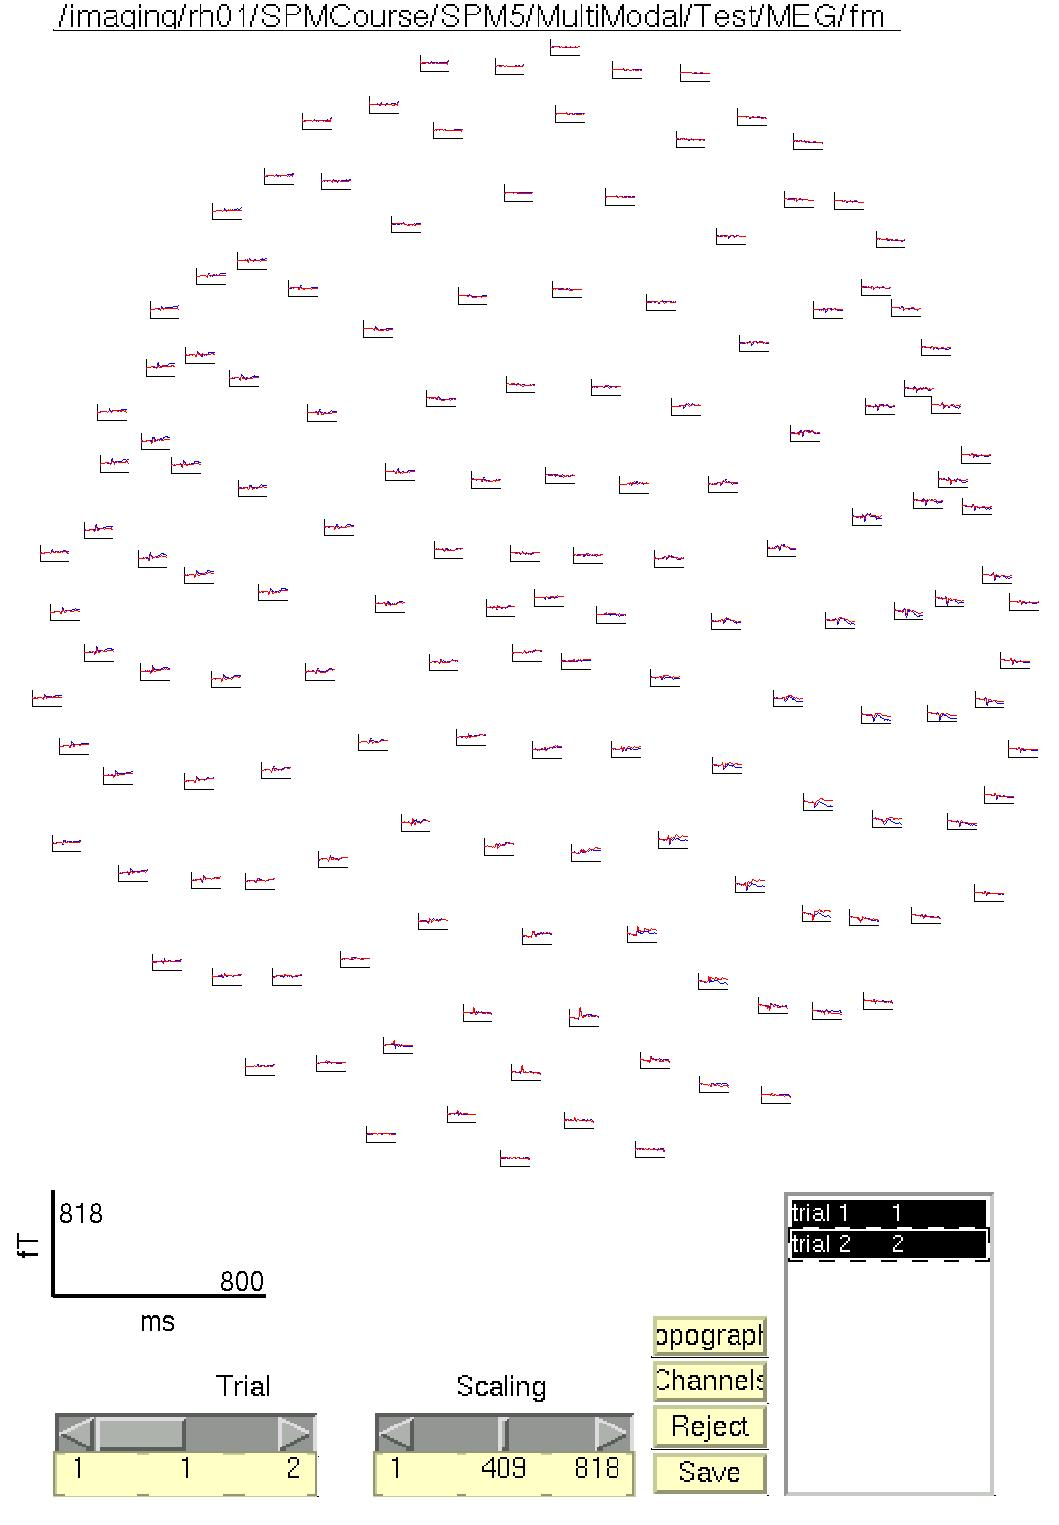
\includegraphics[width=100mm]{multimodal/figures/figure_32_10}
\caption{\em SPM Display window for mean, smoothed ERF (fmcdbespm8_SPM_CTF_MEG_example_faces1_3D.mat) for all 275 MEG channels. \label{fig_32_10}}
\end{center}
\end{figure}


* Select "Contrast" from the "Other..." pulldown menu on the SPM window (or type \verb!spm_eeg_weight_epochs! in the Matlab window). This function creates linear contrasts of ERPs/ERFs. Select the \verb!fmcdbespm8_SPM_CTF_MEG_example_faces1_3D.mat! file, enter $[1 -1]$ as the first contrast and label it 'Difference', answer 'yes' to 'Add another',  enter $[1/2 1/2]$ as the second contrast and label it 'Mean'. Press "no" to the question 'Add another' and not to "weight by num replications". This will create new file \verb!wfmcdbespm8_SPM_CTF_MEG_example_faces1_3D.mat!, in which the first trial-type is now the differential ERF between faces and scrambled faces, and the second trial-type is the average ERF for faces and scambled faces.

To see the topography of the differential ERF, click on Trial 1 again, press the "topography" button at the top of the window and scroll to 165ms for the latency to produce Figure~\ref{fig_32_5}.

You can move the slider left and right to see the development of the M170 over time.

\begin{figure}
\begin{center}
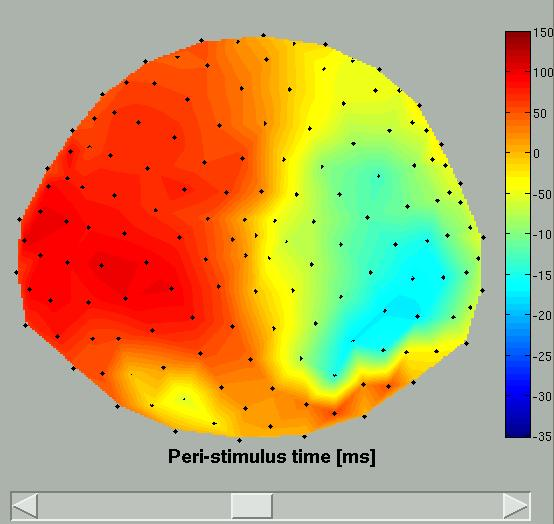
\includegraphics[width=100mm]{multimodal/figures/figure_32_12}
\caption{\em 2D topography of the ERF of faces minus scrambled faces at 165ms\label{fig_32_12}}
\end{center}
\end{figure}

\subsection{Time-Frequency Analysis}

SPM uses Morlet wavelets to perform time-frequency analyses.

* Select the 'time-frequency' option under the 'Other' pull-down menu, and select the \verb!cdbespm8_SPM_CTF_MEG_example_faces1_3D.mat! file. SPM will then prompt you for the frequencies you wish to analyse, for which you can type [5:40] (Hz). To the question "remove baseline", press "no" (because for frequencies as low as 5Hz, one would need a longer pre-stimulus baseline, to avoid edge-effects\footnote{For example, for 5Hz, one would need at least N/2 x 1000ms/5, where N is the order of the Morlet wavelets (i.e, number of cycles per Gaussian window), e.g, 600ms for a 6th-order wavelet.}). Later, we will compare two trial-types directly, and hence any pre-stimulus differences will become apparent. Change the default Morlet wavelet order (N) from 7 to 5. This factor effectively trades off frequency vs time resolution, with a lower order giving higher temporal resolution. You will then be prompted to select channels, for which you can highlight and delete the default option of all channels, and type just 114 (which corresponds to channel 'MLT34', as can be confirmed by typing D.indchannel('MLT34') in the Matlab window)\footnote{You can of course obtain time-frequency plots for every channel, but it will take much longer (and result in a large file).}. Answer 'yes' to 'Compute phase?'.

This will produce two new datasets, \verb!tf1_cdbespm8_SPM_CTF_MEG_example_faces1_3D! and  \verb!tf2_cdbespm8_SPM_CTF_MEG_example_faces1_3D!. The former contains the power at each frequency, time and channel; the latter contains the corresponding phase angles.

* Press the 'Averaging' button and select the \verb!tf1_cdbespm8_SPM_CTF_MEG_example_faces1_3D.mat! file. You can again use robust averaging to compute the average time-frequency representation.
New file will be created in the CTF MEG directory called \verb!mtf1_cdbespm8_SPM_CTF_MEG_example_faces1_3D!. Note that you can use the reviewing tool to review the time-frequency datasets and the corresponding robust averaging weights.

This contains the power spectrum averaged over all trials, and will include both "evoked" and "induced" power. Induced power is (high-frequency) power that is not phase-locked to the stimulus onset, which is therefore removed when averaging the amplitude of responses across trials (i.e, would be absent from a time-frequency analysis of the \verb!mcdbespm8_SPM_CTF_MEG_example_faces1_3D.mat! file).

The power spectra for each trial-type can be displayed using the usual Display button and selecting the \verb!mtf1_cdbespm8_SPM_CTF_MEG_example_faces1_3D.mat! file. This will produce a plot of power as a function of frequency (y-axis) and time (x-axis) for Channel MLT34. If you use the "trial" slider to switch between trial(types) 1 and 2, you will see the greater power around 150ms and 10Hz for faces than scrambled faces (click on one channel to get scales for the axes, as in Figure~\ref{fig_32_13}). This corresponds to the M170 again.


\begin{figure}
\begin{center}
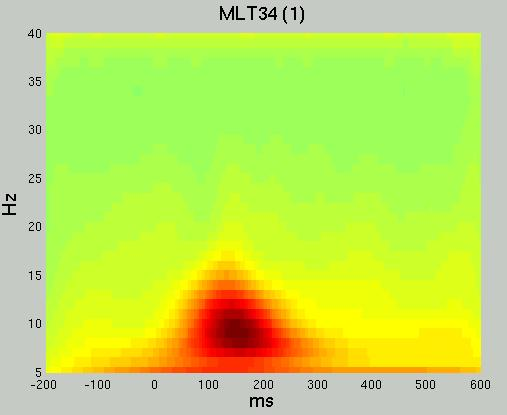
\includegraphics[width=60mm]{multimodal/figures/figure_32_13_L}
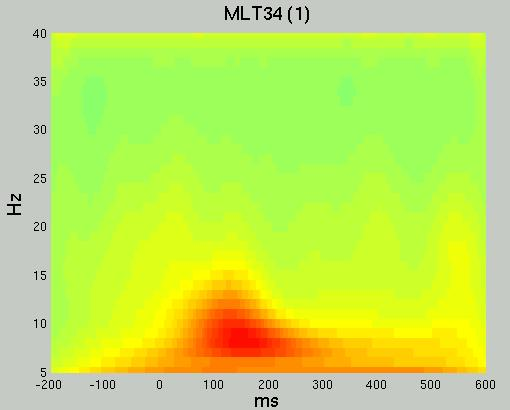
\includegraphics[width=60mm]{multimodal/figures/figure_32_13_R}
\caption{\em  Total power spectra for faces (left) and scrambled faces (right) for channel MLT34\label{fig_32_13}}
\end{center}
\end{figure}

We can also look at evidence of phase-locking of ongoing oscillatory activity by averaging the phase angle information. This time, we do not take the straight (arithmetric) mean, since the data are phase angles, and this average is not particularly meaningful. Instead we calculate their vector mean (when converting the angles to vectors in Argand space), which corresponds to a "Phase-Locking Value" (PLV) which lies between 0 (no phase-locking across trials) to 1 (perfect phase-locking).

* Press the 'Averaging' button and select the \verb!tf2_cdbespm8_SPM_CTF_MEG_example_faces1_3D.mat! file. This time you will be prompted for either a straight or a vector average, for which you should select "Vector (PLV)". The matlab window will echo:
\begin{verbatim}
  mtf2_cdbespm8_SPM_CTF_MEG_example_faces1_3D.mat: Number of replications per contrast:
  average faces: 168 trials, average scrambled: 168 trials
\end{verbatim}
    
and a new file will be created in the MEG directory called \verb!mtf2_cdbespm8_SPM_CTF_MEG_example_faces1_3D.mat!.

If you now display the file \verb!mtf2_cdbespm8_SPM_CTF_MEG_example_faces1_3D.mat! file, you will see PLV as a function of frequency (y-axis) and time (x-axis) for Channel MLT34. Again, if you use the "trial" slider to switch between trial(types) 1 and 2, you will see greater phase-locking around 10Hz and 100ms for faces than scrambled faces, as in Figure~\ref{fig_32_14}. Together with the above power analysis, these data suggest that the M170 includes an increase both in power and in phase-locking of ongoing oscillatory activity in the alpha range (Henson et al, 2005b).


\begin{figure}
\begin{center}
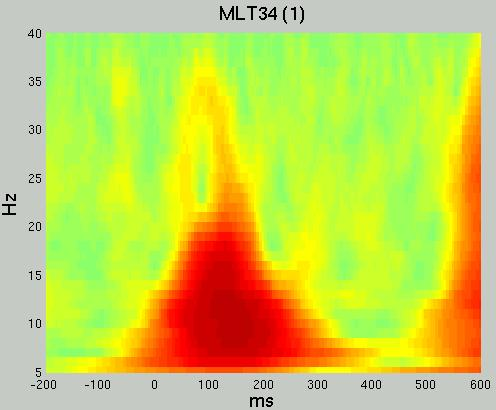
\includegraphics[width=60mm]{multimodal/figures/figure_32_14_L}
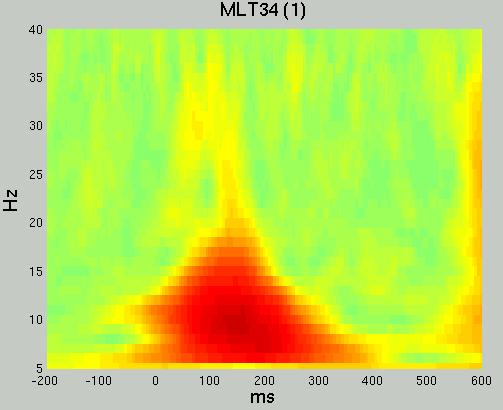
\includegraphics[width=60mm]{multimodal/figures/figure_32_14_R}
\caption{\em Phase-Locking Values for faces (left) and scrambled faces (right) for channel MLT34 \label{fig_32_14}}
\end{center}
\end{figure}

\subsection{2D Time-Frequency SPMs}

Analogous to Section~\ref{3DSPM}, we can also use Random Field Theory to correct for multiple statistical comparisons across the 2-dimensional time-frequency space.

* Select 'Convert to images' in the Matlab window, and select the \verb!tf1_cdbespm8_SPM_CTF_MEG_example_faces1_3D.mat! file.

This will create time-frequency images for each trial of the two types, with dimensions 161x36x1, as for the example shown in Figure~\ref{fig_32_15} from pressing "Display: images" on the main SPM window.

\begin{figure}
\begin{center}
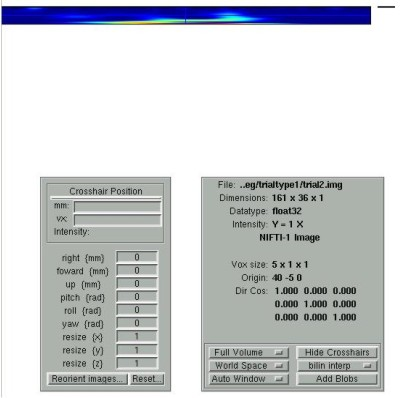
\includegraphics[width=100mm]{multimodal/figures/figure_32_15}
\caption{\em  3D image for trial 2 of t1-e-eeg.mat. The left section is through time (x) and frequency (y) (the right image is an y-z section, though there is only one value in z, i.e, it is really a 2D image).\label{fig_32_15}}
\end{center}
\end{figure}

As in Section~\ref{3DSPM}, we then take these images into an unpaired t-test across trials to compare faces versus scrambled faces. We can then use classical SPM to identify times and frequencies in which a reliable difference occurs, correcting across the multiple comparisons entailed (Kilner et al, 2005).

* First create a new directory, eg. mkdir TFstatsPow.

* Then press the "specify 2nd level" button,  select "two-sample t-test" (unpaired t-test), and define the images for "group 1" as all those in the subdirectory "trialtype1" (using right mouse, and "select all") and the images for "group 2" as all those in the subdirectory "trialtype2". Finally, specify the new TFstatsPow directory as the output directory, and press "run". (Note that this will be faster if you saved and could load an SPM job file from Section~\ref{3DSPM}).

This will produce the design matrix for a two-sample t-test.

* The press "Estimate", and when it has finished, press "Results" and define a new T-contrast as [1 -1]. Keep the default contrast options, but threshold at $p<.05$ FWE corrected for the whole "image". Then press "whole brain", and the Graphics window should now look like that in Figure~\ref{fig_32_16} (ignore the glass brain MIP).


\begin{figure}
\begin{center}
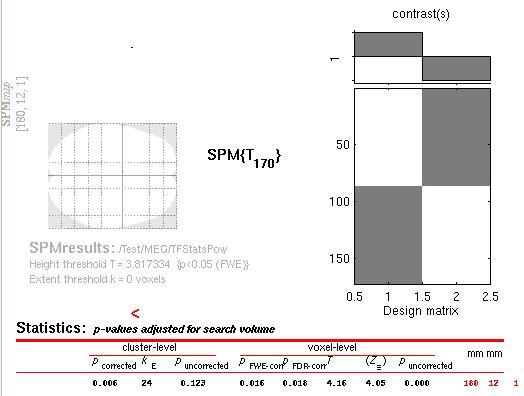
\includegraphics[width=100mm]{multimodal/figures/figure_32_16}
\caption{\em  2D time-frequency SPM{T} at $p<.001$ uncorrected for the power difference between face and scrambled faces at Channel MLT34. Note that the brain outline in the MIP should be ignored. The x  coordinates refer to time in ms; the y coordinates refer to frequency in Hz (the z-coordinate is always 1).\label{fig_32_16}}
\end{center}
\end{figure}

This will list one "region" within the 2D time-frequency space in which faces produce greater power than scrambled faces, having corrected for multiple T-tests across pixels. This has a maximum of  [180 12 1], ie 12 Hz and 180ms post-stimulus.

If you repeat the above time-frequency analysis on the \verb!cdbespm8_SPM_CTF_MEG_example_faces1_3D.mat! file, but this time keep every channel and answer 'yes' to the "average over channels?" question, and then repeat the above statistical analysis of power, you will notice that there is also a reliable decrease in induced high-frequency power (around 400ms and 35 Hz) for faces vs scrambled faces, which could also be source-localised.


\subsection{"Imaging" reconstruction of differential power}

In Section~\ref{3D} we localised the differential evoked potential difference in EEG data corresponding to the N170.  Here we will localise the total power of faces vs scrambled faces in a timewindow corresponding to that of the M170, ie including potential induced components (see Friston et al, 2000).

* Press the '3D source reconstruction' button, and press the "load" button at the top of the new window. Select the \verb!cdbespm8_SPM_CTF_MEG_example_faces1_3D.mat! file and type a label (eg "M170") for this analysis.

* Press the 'MRI' button, select the smri.img file within the sMRI sub-directory and select the 'normal' mesh.

If you have not used this MRI image for source reconstruction before, this step will take some time while the MRI is segmented and the deformation parameters computed (see Section~\ref{3D} for more details on these files). When meshing has finished, the cortex (blue), inner skull (red) and scalp (orange) meshes will also be shown in the Graphics window with slices from the sMRI image. This makes it possible to verify that the meshes indeed fit the original image well. The field D.inv\{1\}.mesh field will be updated in matlab. Press "save" in top right of window to update the corresponding mat file on disk.

Both the cortical mesh and the skull and scalp meshes are not created directly from the segmented MRI, but rather are determined from template meshes in MNI space via inverse spatial normalisation (Mattout et al, in press).

* Press the 'Co-register' button. You will be asked for each of the 3 fiducial points to specify its location on the MRI images. This can be done by  selecting a corresponding point from a hard-coded list ('select'). These points are inverse transformed for each individual image using the same deformation field that is used to create the meshes. The other two options are typing the MNI coordinates for each point ('type') or clicking on the corresponding point in the image ('click'). You can either use the 'select' option and just press OK for each point as SPM automatically selects a point with the same name or open the \verb!smri_fid.txt! file located in the sMRI directory and use the 'type' option copying the locations from there. Answer 'no' to 'Use headshape points?'.

This stage coregisters the EEG sensor positions with the structural MRI and cortical mesh, via an approximate matching of the fiducials in the two spaces, followed by a more accurate surface-matching routine that fits the head-shape function (measured by Polhemus) to the scalp that was created in the previous meshing stage via segmentation of the MRI. When coregistration has finished, the field D.inv\{1\}.datareg will be updated in matlab. Press "save" in top right of window to update the corresponding mat file on disk. Finally, a figure like that in Figure~\ref{fig_32_8} will also be produced, which you can rotate with the mouse (using the Rotate3D Matlab Menu option) to check all sensors.

In this case since the fiducial locations measured are quite precise fitting the headshape to headsurface actually impairs the quality of the coregistration (you can try). So it'd be better to just inspect the headshape points visually and make sure that they make sense.


\begin{figure}
\begin{center}
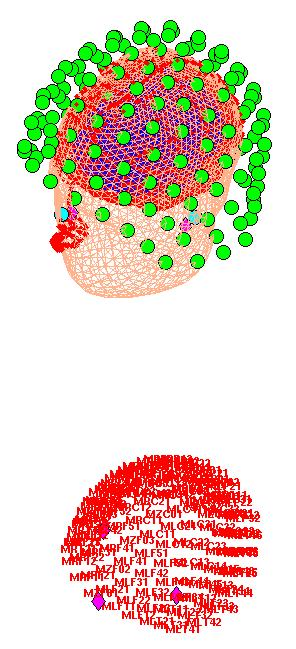
\includegraphics[width=70mm]{multimodal/figures/figure_32_17}
\caption{\em  Graphical output of registration of MEG and sMRI data, showing (upper panel) cortex (blue) and scalp (black) meshes, sensor locations (green), MRI and Polhemus fiducials (cyan/magneta), and headshape (red dots).\label{fig_32_17}}
\end{center}
\end{figure}


* Press the 'Forward Model' button. Choose 'Single shell' (you may also try the other options). A figure will be displaying showing the head model, the cortical mesh and the sensors. 


* Press 'Invert.', select 'Imaging', select 'yes' to 'All conditions or trials?', and "Standard" for the model (i.e, to use defaults; you can customise a number of options if you press Custom instead) (see Friston et al, in press-a, for more details about these parameters). There will be lead field computation followed by the actual inversion and a plot of summary of the results will be displayed at the end. 

Press "save" to save the results. You can now explore the results via the 3D reconstruction window. If you type 165 into the box in the bottom right (corresponding to the time in ms) and press "mip", you should see an output like in Figure~\ref{fig_32_18}.

Note the hot-spots in the fusiform. The timecourses come from the peak voxel. The red line shows the condition currently being shown (corresponding to the "Condition 1" toggle bar in the reconstruction window); the grey line(s) will show all other conditions. Condition 1 is faces; if you press the "condition 1" toggle, it will change to Condition 2 (scrambled faces), then press "mip" again and the display will update (note the colours of the lines have now reversed from before, with red now corresponding to scrambled faces).

If you toggle back to condition 1 and press "movie", you will see the changes in the source strengths over peristimulus time (from the limits 0 to 300ms currently chosen by default).

If you press "render" you can get a very neat graphical interface to explore the data (the buttons are fairly self-explanatory). However, we will concentrate on how one might perform statistics.


\begin{figure}
\begin{center}
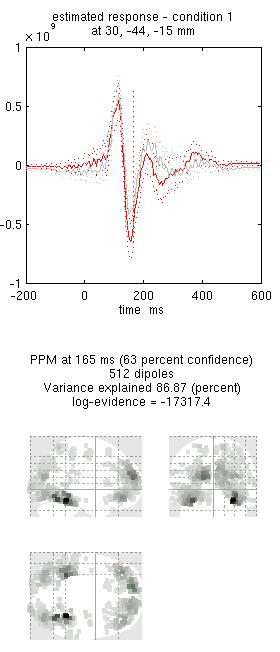
\includegraphics[width=90mm]{multimodal/figures/figure_32_18}
\caption{\em  Graphic output for MSP-estimated activity at 165ms for faces.\label{fig_32_18}}
\end{center}
\end{figure}

* Press the "Window" button in the reconstruction window, enter "150 200" as the timewindow of interest and "5 40" as the frequency band of interest. Then choose the 'induced' option. After a delay the Graphics window will show the mean activity for this time/frequency contrast (for faces alone, assuming the condition toggle is showing "condition 1").

* If you then press "Image", press "12" for the smoothing kernel, and SPM will write 3D Nifti images corresponding to the above contrast for each condition:
\begin{verbatim}
    w_cdbespm8_SPM_CTF_MEG_example_faces1_3D_1_1.nii
    w_cdbespm8_SPM_CTF_MEG_example_faces1_3D_1_2.nii
    sw_cdbespm8_SPM_CTF_MEG_example_faces1_3D_1_1.nii
    sw_ecdbespm8_SPM_CTF_MEG_example_faces1_3D_1_2.nii
\end{verbatim}
Note that the first two images are unsmoothed (but normalised); the latter two are smoothed by a 12mm isotropic Gaussian kernel. The last number in the file name refers to the condition number; the penultimate number refers to the reconstruction number (ie the number in red in the reconstruction window, i.e, D.val, here 1).

The smoothed results for Condition 1 will also be displayed in the Graphics window, together with the normalised structural, as in Figure~\ref{fig_32_19}. Note that the solution image is in MNI (normalised) space, because the use of a canonical mesh provides us with a mapping between the cortex mesh in native space and the corresponding MNI space.

You can also of course view the image with the normal SPM "Display:image" option, and locate the coordinates of the "hotspots" in MNI space. Note that these images contain RMS (unsigned) source estimates (see Henson et al, 2007).

If you want to see where activity (in this time/freq contrast) is greater for faces and scrambled faces, you can use SPM's ImCalc to create a difference image of \verb!sw_cdbespm8_SPM_CTF_MEG_example_faces1_3D_1_1.nii - sw_cdbespm8_SPM_CTF_MEG_example_faces1_3D_1_2.nii! - you should see bilateral fusiform. For further discussion of localising a differential effect (as in Section~\ref{3D} with ERPs), vs taking the difference of two localisations, as here, see Henson et al (2007).

    

\begin{figure}
\begin{center}
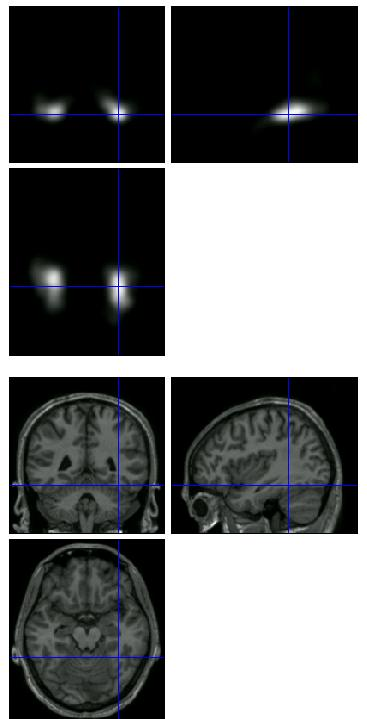
\includegraphics[width=100mm]{multimodal/figures/figure_32_19}
\caption{\em  Display of the smoothed 3D image of the MSP-estimated activity between 150-200ms in the frequency band 5-40Hz for faces, together with the normalised structural. Note large hotspots in bilateral fusiform.\label{fig_32_19}}
\end{center}
\end{figure}

You could also explore the other inversion options, like COH and MNM, which you will note give more superficial solutions (a known problem with standard minimum norm; see also Friston et al, in press-a). To do this quickly (without repeating the MRI segmentation, coregistration and forward modelling), press the "new" button in the reconstruction window, which by default will copy these parts from the previous reconstruction.


\section{fMRI analysis \label{fMRI}}

Only the main characteristics of the fMRI analysis are described below; for a more detailed demonstration of fMRI analysis, see Chapter 29.

Note that all the job files for each stage of preprocessing and analysis are also provided:
\begin{verbatim}
    fMRI/realign_job.mat
    fMRI/slicetime_job.mat
    fMRI/smooth_job.mat
    fMRI/stats_job.mat
\end{verbatim}
These can be loaded and run, though of course the location of the files and the output directory will need to be changed.

\subsection{Preprocessing the fMRI data}

* Toggle the modality from EEG to fMRI, and change directory to the fMRI subdirectory (either in Matlab, or via the "CD" option in the SPM "Utils" menu)

* Select 'Realign' from the 'Realign and Unwarp' menu, click on 'Data', and select 'New Session'. Double-click on the new Session branch, and click on the 'Images' button, click on the 'specify files' and select all 215 \verb!fM*.img! files in the Scan directory (using the right mouse to 'select all', assuming the filter is set to \verb!^f.*img!).

Realignment will produce a \verb!spm*.ps! postscript file in the current directory, which shows the estimated movement (like in Figure~\ref{fig_32_20}). Importantly, the resliced images will be output as rfM*.img files. A mean image will also be written:
\begin{verbatim}
        meanfMS02554-0003-000006.img
\end{verbatim}
as will the movement parameters in the text file:
\begin{verbatim}
        rp_fMS02554-0003-000006.txt
\end{verbatim}

.
\begin{figure}
\begin{center}
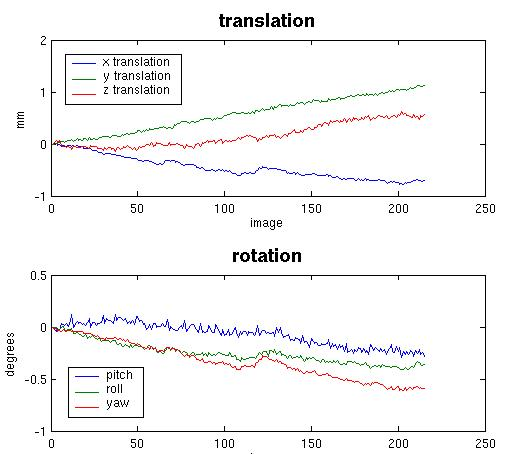
\includegraphics[width=100mm]{multimodal/figures/figure_32_20}
\caption{\em  Movement parameters from Realignment of the fMRI data. \label{fig_32_20}}
\end{center}
\end{figure}

* Press the 'slice-timing' button, select the functional images (filter set to \verb!^rf.*! to avoid the mean image), enter 2.88 as the TR, 2.88*31/32 as the TA, the slice-order as [1:32] (since the first slice in the file is the top slice, and this was the first slice acquired in the descending sequence), and the reference slice to 16. This will write out 215 images arfM*.img, in which the data have been interpolated to match the acquisition time of the middle slice (in space and time, given the sequential acquisition).

* Press the 'smooth' button and keep the default 10x10x10mm smoothing. This will produce 215 spatially-smoothed images sarfM*.img.

Note that we will not normalise these images, in order to compare them with the MEG and EEG source reconstructions, which are in the native MRI space.

\subsection{Statistical analysis of fMRI data}

* Load the onsets.mat file provided into the Matlab workspace

* Press the 'specify 1st-level' button, change the microtime onset from 1 to 8, select the 215 'sarfM*img' images, define two new conditions - condition 1 called "faces" with onsets set to onsets{1} and condition 2 called "scrambled faces" with onsets set to onsets{2} (all duration 0) - select the  \verb!rp_fMS02554-0003-000006.txt! file as 'Multiple Regressors' (to covary out some of the residual movement-related effects), and select the fMRI/Stats as the output directory (loading and editing the \verb!stats_job.mat! file provided will save a lot of time here!). Keep the rest of the parameters (e.g, use of a canonical HRF basis function) at their default settings.

This will produce a design matrix like that in Figure~\ref{fig_32_21}, which is stored in the file:
\begin{verbatim}
        fMRI/Stats/SPM.mat
\end{verbatim}

\begin{figure}
\begin{center}
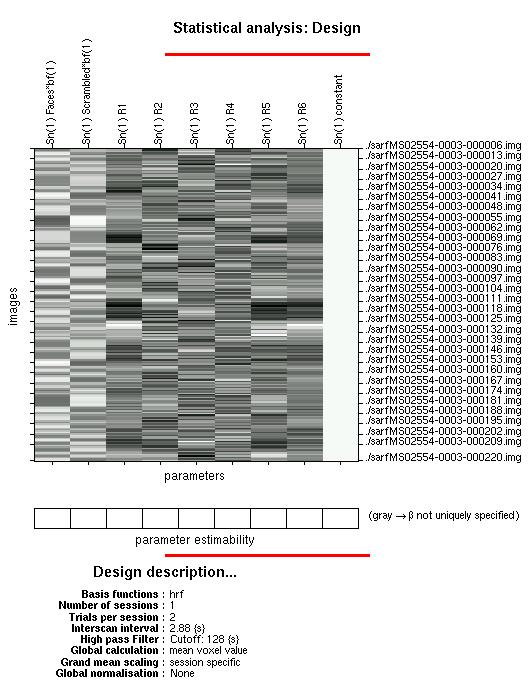
\includegraphics[width=100mm]{multimodal/figures/figure_32_21}
\caption{\em Design matrix for the fMRI analysis. \label{fig_32_21}}
\end{center}
\end{figure}

* Then estimate the parameters of the design matrix by pressing the 'Estimate' button and selecting the SPM.mat file

* Finally, to see the regions that respond differentially between faces and scrambled faces, press 'Results' and define a new F-contrast (called, e.g, 'Faces - Scrambled') by typing the contrast weights [1 -1].

This will identify regions in which the parameter estimate for the canonical HRF differs reliably between faces and scrambled faces. This could include regions that show both a "greater" relative response for faces, and regions that show a "greater" relative response for scrambled faces (such a two-tailed test is used because we do not know the precise relationship between haemodynamic changes measured by fMRI and the synchronous current changes measured by EEG/MEG).

If the resulting SPM{F} is thresholded at $p<.05$ FWE corrected, the resulting MIP and table of values should be like that in Figure ~\ref{fig_32_22}. Only two regions survive correction: right fusiform and orbitofrontal cortex (note coordinates refer to native MRI space; not MNI space). These can be displayed on the (attentuation-corrected) structural msmri.nii. They are a subset of the regions identified by the same contrast in a group of 18 subjects in Henson et al (2003). At a lower threshold (e.g, $p<.01$ uncorrected), one can see additional activation in left fusiform, as well as other regions.


\begin{figure}
\begin{center}
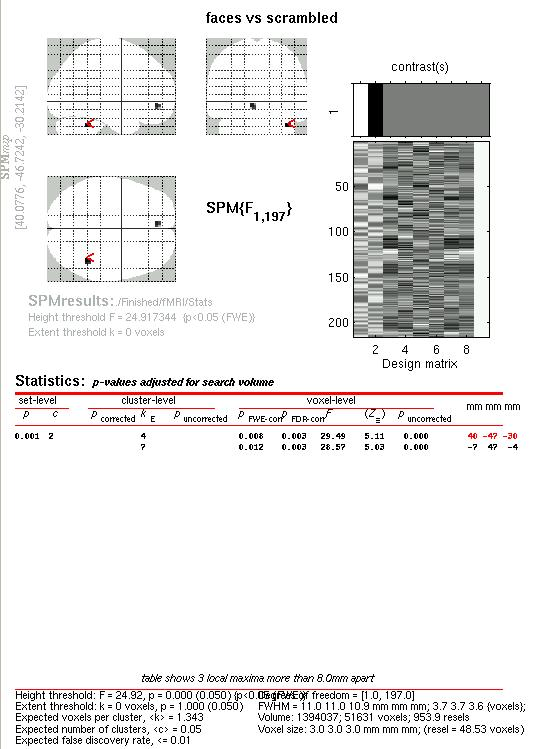
\includegraphics[width=100mm]{multimodal/figures/figure_32_22}
\caption{\em  SPM{F} for faces vs scrambled faces. Note that the coordinates are in the MRI native space (no normalisation performed) so bear a close, but not exact, relationship with MNI coordinates (affecting brain outline in MIP too).\label{fig_32_22}}
\end{center}
\end{figure}

There is some agreement between these fMRI effects and the localised EEG/MEG effects around the 170ms latency - eg in orbitofrontal and right fusiform - though of course the EEG dipoles were bilateral, and there were more extensive posterior occipitotemporal effects in the source-localised MEG data. Note of course that the fMRI data may include differences between faces and scrambled faces that occur at latencies other than the M170 (e.g, later), or differences in "induced" high-frequency M/EEG power that is not phase-locked to stimulus onset (Henson et al, 2005b).

One could use the unthresholded F-image as an additional continuous prior within the PEB L2-norm method offered by SPM5, or probably better, one could take a number of regions after thresholding the SPM{F}, and enter each as a separate prior on the PEB L2-norm method (this way, different regions can be up-weighted or down-weighted as a function of whether they are likely to be active during the critical timewindow being localised).



\section{References}

\noindent 1. Friston, K, Daunizeau, J, Kiebel, S, Phillips, C, Trujillo-Barreto, N, Henson, R, Flandin, G, Mattout, J (in press-a). Multiple sparse priors for the M/EEG inverse problem. Neuroimage. \\

\noindent 2. Friston, K, Carlton Chu, Janaina Mouro-Miranda, Oliver Hulme, Geraint Rees, Will Penny and John Ashburner (in press-b). Bayesian decoding of brain images. NeuroImage.\\

\noindent 3. Friston K, Henson R, Phillips C, and Mattout J. (2006). Bayesian estimation of evoked and induced responses. Human Brain Mapping, 27, 722-735.\\

\noindent 4. Henson, R, Goshen-Gottstein, Y, Ganel, T, Otten, L, Quayle, A. and Rugg, M. (2003). Electrophysiological and hemodynamic correlates of face perception, recognition and priming. Cerebral Cortex, 13, 793-805.\\

\noindent 5. Henson R, Mattout J, Friston K, Hassel S, Hillebrand A, Barnes G and Singh K. (2005a) Distributed source localisation of the M170 using multiple constraints. HBM05 Abstract.\\

\noindent 6. Henson R, Kiebel S, Kilner J, Friston K, Hillebrand A, Barnes G and Singh K. (2005b) Time-frequency SPMs for MEG data on face perception: Power changes and phase-locking. HBM05 Abstract.\\

\noindent 7. Henson, R.N. Mattout, J, Singh, K, Barnes, G, Hillebrand, A. and Friston, K.J. (2007). Population-level inferences for distributed MEG source localisation under multiple constraints: Application to face-evoked fields. Neuroimage, 38, 422-438.\\

\noindent 8. Josephs, O., Deichmann, R., Turner, R. (2000). Trajectory measurement andgeneralised reconstruction in rectilinear EPI. NeuroImage 11, S543.\\

\noindent 9. Kilner, J., Kiebel, S and Friston, K. J. (2005). Applications of random field theory to electrophysiology. Neuroscience Letters, 374:174-178.\\

\noindent 10. Kilner, J. and Penny. W. (2006). Robust Averaging for EEG/MEG. HBM06 Abstract.\\

\noindent 11. Kiebel S and Friston K (2004). Statistical Parametric Mapping for Event-Related Potentials II: A Hierarchical Temporal Model. NeuroImage, 22, 503-520.\\

\noindent 12. Kiebel, S.J., David, O. and Friston, K. J. (2006). Dynamic Causal Modelling of Evoked Responses in EEG/MEG with lead-field parameterization. NeuroImage, 30:1273-1284.\\

\noindent 13. Mattout J, Pelegrini-Issac M, Garnero L and Benali H. (2005a). Multivariate source prelocalization (MSP): use of functionally informed basis functions for better conditioning the MEG inverse problem. Neuroimage, 26, 356-73.\\

\noindent 14. Mattout, J, Phillips, C, Penny, W, Rugg, M and Friston, KJ (2005b). MEG source localisation under multiple constraints: an extended Bayesian framework. NeuroImage.\\

\noindent 15. Mattout, J., Henson, R N. and Friston, K.J. (in press). Canonical Source Reconstruction for MEG. Computational Intelligence and Neuroscience.\\

\noindent 16. Phillips, C. M.D. Rugg, M and Friston, K (2002). Systematic Regularization of Linear Inverse Solutions of the EEG Source Localisation Problem. NeuroImage, 17, 287-301.\\

\noindent 17. Spinelli, L, Gonzalez S, Lantz, G, Seeck, M and Michel, C. (2000). Electromagnetic inverse solutions in anatomically constrained spherical head models. Brain Topography, 13, 2.\\

